\documentclass[letterpaper]{article}

\usepackage[margin=1in]{geometry}
\usepackage{amsmath,amssymb,amsthm}
\usepackage{booktabs}
\usepackage{graphicx}
\usepackage{natbib}
\usepackage{hyperref}
\usepackage{xcolor}
\usepackage{pifont}
\usepackage{multirow}

\newtheorem{definition}{Definition}
\newtheorem{proposition}{Proposition}
\newtheorem{theorem}{Theorem}
\newtheorem{lemma}{Lemma}

\graphicspath{{../../figures/paper/}}

\title{Multi-Class Annotation Errors in Causal Inference:\\Topology-Dependent Bias, Sensitivity, and Correction}

\author{}
\date{}

\begin{document}
\maketitle

\begin{abstract}
Large language models (LLMs) are increasingly used as annotators in computational social science, yet annotation errors propagate into downstream causal estimates in ways that binary measurement error theory cannot predict. We present the first systematic framework characterizing how $K$-class confusion matrix structure interacts with DAG topology to determine bias direction and magnitude. We derive bias expressions for seven canonical DAG topologies under multi-class non-differential misclassification (closed-form for confounding, exposure, and mediation; numerically validated for all seven) and establish a structural sign-flip guarantee (with formal proofs for three topologies and Monte Carlo validation for all seven): five topologies (confounding, mediation, collider, M-bias, front-door) never produce sign reversal regardless of the confusion matrix, while exposure and instrumental variable topologies can. In the exposure DAG, 83.4\% of $K{=}3$ confusion matrices cause sign reversal, a failure that persists at 13.7\% violation rate (2.1\% sign reversal, 11.7\% amplification) even with classifier accuracy above 70\%. We introduce Annotation Sensitivity Values (ASVs), a sensitivity analysis framework with three complementary measures that reveal a topology-dependent vulnerability spectrum: IV estimates are maximally vulnerable (52.6\% sign reversal; sign-flip ASV $= 1.1$--$6.7$) while M-bias adjustment is immune (ASV $= \infty$). We evaluate five correction methods across all topologies and prove a Frisch--Waugh--Lovell invariance result: matrix-based corrections achieve 0\% bias reduction on the target coefficient for four topologies, while PPI++ achieves 93.8\% reduction but requires gold labels. Binarization from multi-class to binary introduces additional bias varying 147$\times$ across topologies. Neither classification $F_1$ nor correction method choice alone determines downstream safety; topology-aware analysis is necessary for valid causal inference with LLM-generated annotations.
\end{abstract}


\section{Introduction}
\label{sec:introduction}

Large language models are rapidly replacing human annotators in computational social science, with researchers using LLM-generated labels for tasks ranging from sentiment classification to political stance detection~\cite{egami_hinck_stewart_wei2023, baumann2025}. This shift promises dramatic cost reduction, but introduces a critical validity gap: annotation errors from imperfect classifiers propagate into downstream causal estimates in ways that depend on both the error structure and the causal design. \citet{baumann2025} demonstrate that across 37 annotation tasks, 31\% of hypotheses yield incorrect conclusions with state-of-the-art LLMs, rising to 50\% for smaller models. Even classifiers achieving $F_1 > 0.93$ produce over 50\% downstream error risk.

The consequences can be catastrophic. Under $K{=}3$ non-differential exposure misclassification, 83.4\% of confusion matrices cause \emph{sign reversal} of the estimated treatment effect, where the estimated direction of the causal relationship is opposite to the truth. This failure breaks the classical binary guarantee that non-differential misclassification biases estimates ``toward the null''~\cite{brenner1993}, a guarantee that many applied researchers implicitly rely upon. The breakdown is not an edge case: it persists even when classifier accuracy exceeds 70\% (13.7\% violation rate at diagonal $\geq 0.7$, comprising 2.1\% sign reversal and 11.7\% amplification).

Why does the multi-class setting behave so differently? For binary classification, non-differential error can only attenuate the effect because the $2{\times}2$ stochastic confusion matrix preserves coefficient signs. With $K \geq 3$ categories, the confusion matrix can assign negative effective weights to categories with opposite-sign coefficients, enabling sign reversal~\cite{veirod_laake2001}. This fundamental asymmetry between binary and multi-class annotation error has received limited systematic treatment. \citet{brenner1993} identified the possibility of polytomous reversal but did not characterize it across causal designs. \citet{lee_wood_doughty2024} extended classifier error analysis to categorical variables and LLM classifiers, but covered only one DAG topology (unobserved confounding). No existing framework addresses how the same confusion matrix produces qualitatively different bias across different causal identification strategies.

Compounding this gap, \citet{kim_garg2025} show that LLM errors are highly correlated across models (60\% agreement when both err), undermining the common assumption that ensembling multiple LLMs can mitigate annotation error. This finding strengthens the case that analyzing the \emph{structure} of annotation error, rather than simply reducing its magnitude, is essential for valid downstream inference.

We address these gaps with three contributions:

\begin{enumerate}
\item \textbf{Multi-class bias taxonomy.} We derive bias expressions for seven canonical DAG topologies (Figure~\ref{fig:dag_taxonomy}) under $K$-class non-differential misclassification (closed-form for confounding, exposure, and mediation; numerically validated for all seven). We establish that five topologies maintain a structural sign-flip guarantee (with formal proofs for three topologies and Monte Carlo validation for all seven) ($\tau_{\text{sign\_flip}} = 0$), while exposure and IV topologies can produce sign reversal. This taxonomy reveals that bias direction is determined by the \emph{interaction} between the confusion matrix and the DAG topology, not by either alone.

\item \textbf{Annotation Sensitivity Values (ASVs).} We propose a unified sensitivity analysis framework with three complementary measures: magnitude ASV (E-value analogue for annotation error), significance ASV (hypothesis test filter for attenuating topologies), and sign-flip ASV (for exposure and IV). ASVs reveal a vulnerability spectrum from IV (maximally fragile, 52.6\% sign reversal; sign-flip ASV $= 1.1$--$6.7$) to M-bias (immune, ASV $= \infty$), providing practitioners with topology-aware robustness diagnostics.

\item \textbf{Topology-aware correction guidance.} We evaluate five correction methods (naive plug-in, MLA, DSL, MC-SIMEX, PPI++) across all seven topologies and show that correction effectiveness is itself topology-dependent. A Frisch--Waugh--Lovell invariance result proves that matrix-based corrections achieve exactly 0\% bias reduction on the target coefficient for four topologies, while PPI++ achieves 93.8\% bias reduction but requires gold-standard labels. We further show that collapsing $K{=}3$ annotations to binary introduces additional bias varying 147$\times$ across topologies.
\end{enumerate}


\section{Related Work}
\label{sec:related_work}

\paragraph{Measurement error in causal inference.}
The epidemiology literature has long studied misclassification bias through causal diagrams~\cite{gustafson2004}. \citet{hernan_cole2009} formalized the starred-node DAG framework for reasoning about measurement bias, distinguishing differential from non-differential error. For binary variables, \citet{ogburn_vanderweele2012} proved that non-differential confounder misclassification produces adjusted estimates between the crude and true values, precluding sign reversal. \citet{brenner1993} showed this guarantee breaks for polytomous confounders, and \citet{veirod_laake2001} derived bias expressions for multi-category exposure misclassification in Poisson regression. \citet{edwards_lessler_naimi2021} further demonstrated that dependent misclassification of covariate and exposure can bias in either direction. Our work extends this line by providing a systematic taxonomy across seven DAG topologies with closed-form expressions for the $K$-class case, identifying which topologies preserve and which break the sign-flip guarantee.

\paragraph{Text classifier errors in causal studies.}
\citet{wood_doughty2018} first applied DAG reasoning to text classifier measurement error, noting matrix adjustment correction but without formal bias theorems. \citet{teblunthuis2024} provided the most complete binary treatment: four DAG scenarios with testable conditions and a Maximum Likelihood Adjustment method, but restricted to binary classification. \citet{yang_adomavicius2018} formalized the two-stage pipeline problem (data mining followed by econometric analysis) and proved that ML-generated variables systematically bias downstream regression. \citet{keith_jensen_oconnor2020} surveyed the text-and-causal-inference landscape, identifying classifier measurement error as a key open challenge. \citet{lee_wood_doughty2024} extended to categorical LLM classifiers on clinical data but covered only one topology (unobserved confounding). \citet{chen_bhattacharya_keith2024} used zero-shot NLP models as proxies in proximal causal inference, proving identification conditions for one DAG structure. We generalize across all seven topologies with multi-class confusion matrices, providing both bias expressions and sensitivity analysis tools absent from prior work.

\paragraph{LLM annotation quality.}
Recent work has quantified the downstream risks of LLM annotation. \citet{baumann2025} demonstrated across 37 tasks that 31\% of hypotheses yield incorrect conclusions with LLM annotations. \citet{kim_garg2025} showed that LLM errors are 60\% correlated across models, undermining ensemble-based mitigation. \citet{messing2026} decomposed LLM pipeline variance via linear mixed models but explicitly excluded causal identification. \citet{stolwijk_boukes_trilling2025} found that LLM annotations differ from human annotations in prevalence even when per-sample accuracy is adequate, and \citet{cheng_mayya_sedoc2024} decomposed annotation measurement error into four source types. These works diagnose the annotation quality problem; our contribution provides the causal-analytic bridge connecting annotation error structure to downstream causal estimate validity.

\paragraph{Sensitivity analysis for observational studies.}
Our ASV framework draws on the tradition of sensitivity analysis for unmeasured confounding~\cite{rosenbaum2002}. \citet{vanderweele_ding2017} introduced E-values as interpretable sensitivity measures, and \citet{ding_vanderweele2016} developed assumption-free sensitivity bounds. \citet{vanderweele_li2019} extended sensitivity analysis to differential measurement error but only for binary settings. \citet{smith_vanderweele2021} proposed bounds for multiple bias sources including misclassification. Our ASVs adapt the E-value philosophy (``how much bias would be needed to explain away the finding?'') to annotation-induced bias, with three complementary measures tailored to different topology-dependent failure modes.

\paragraph{Correction methods.}
Prediction-powered inference~\cite{angelopoulos2023} and design-based supervised learning~\cite{egami_hinck_stewart_wei2023, gligoric2025} provide general frameworks for valid inference with ML-generated labels, combining predicted labels with small gold-standard samples. \citet{zrnic_candes2024} extended PPI via cross-prediction for improved efficiency. \citet{audinet2025} benchmarked these methods across datasets. These correction methods are complementary to our framework: our topology-dependent ASV analysis identifies \emph{when} correction is needed and \emph{which} failure mode to address, while PPI/DSL provide the \emph{how}.


\section{Method}
\label{sec:method}

\subsection{Setup and Notation}
\label{sec:notation}

Let $A$ denote a true $K$-class categorical variable (e.g., sentiment with $K{=}3$ levels) and $A^*$ its observed, potentially misclassified version produced by an LLM annotator. The misclassification process is characterized by a $K{\times}K$ confusion matrix $C$ with entries $C_{jk} = P(A^*{=}j \mid A{=}k)$, where each column sums to one. Following \citet{hernan_cole2009}, we represent this measurement process using \emph{starred-node} DAGs: the true variable $A$ is latent, and the observed $A^*$ is connected to $A$ via a dashed measurement edge.

\begin{definition}[Non-differential misclassification]
\label{def:nondiff}
Misclassification of $A$ is non-differential with respect to outcome $Y$ and covariates $\mathbf{Z}$ if $P(A^*{=}j \mid A{=}k, Y, \mathbf{Z}) = P(A^*{=}j \mid A{=}k) = C_{jk}$ for all $j,k$.
\end{definition}

We study seven canonical DAG topologies (Figure~\ref{fig:dag_taxonomy})~\cite{pearl2009} in which $A$ occupies structurally distinct causal roles: confounder, exposure, mediator, collider, M-bias variable, front-door mediator, and instrument. Each role induces a different functional relationship between $C$ and the probability limit of the standard causal estimator, yielding topology-dependent bias.

\subsection{Multi-Class Bias Expressions}
\label{sec:bias_expressions}

For each topology, we derive the probability limit of the naive estimator that substitutes $A^*$ for $A$. Let $\tau$ denote the target causal parameter and $\hat{\tau}(A^*)$ the estimator using misclassified annotations.

\paragraph{Confounding ($A$ = confounder).}
When $A$ confounds the $X{\to}Y$ relationship, the OLS estimator controlling for $A^*$ has probability limit
\begin{equation}
\label{eq:confounding}
\text{plim}\;\hat{\tau}(A^*) = \bigl(\mathbb{E}[Z^{\prime}Z]\bigr)^{-1}\mathbb{E}[Z^{\prime}X]\,\boldsymbol{\beta},
\end{equation}
where $Z = [X, \text{dummies}(A^*)]$, $\boldsymbol{\beta}$ contains the true coefficients, and the target parameter $\tau$ is the coefficient on $X$. Misclassification produces residual confounding that monotonically approaches the omitted variable bias, but the sign of $\hat{\tau}$ is preserved: $\tau_{\text{sign\_flip}} = 0$ structurally.

\paragraph{Exposure ($A$ = treatment variable).}
When $A$ is the exposure of interest, the biased coefficient for category $j$ becomes a weighted combination of true coefficients:
\begin{equation}
\label{eq:exposure}
\text{plim}\;\hat{\beta}_j(A^*) = \sum_{k=1}^{K} w_{jk}\,\beta_k,
\end{equation}
where $w_{jk}$ depends on the confusion matrix $C$ and the marginal distribution of $A$. Unlike the binary case, where non-differential misclassification guarantees attenuation toward the null~\cite{brenner1993}, the $K{\geq}3$ case permits $w_{jk}$ to assign negative weight to categories with opposite-sign coefficients, producing \emph{sign reversal}. A near-permutation confusion matrix effectively swaps category labels, making sign reversal the dominant outcome (83.4\% under uniform Dirichlet prior). This failure mode is structurally impossible at $K{=}2$ because a $2{\times}2$ stochastic matrix with positive diagonal cannot reverse the sign of a single coefficient.

\paragraph{Mediation ($A$ = mediator).}
When $A$ mediates the $X{\to}Y$ relationship, the direct effect estimator controlling for $A^*$ has probability limit
\begin{equation}
\label{eq:mediation}
\text{plim}\;\hat{\tau}_{\text{direct}}(A^*) = \tau_{\text{direct}} + \bigl(1 - \lambda(C)\bigr)\,\tau_{\text{indirect}},
\end{equation}
where $\lambda(C) \in [0,1]$ summarizes the weighted attenuation structure (see Appendix~\ref{app:proof}, Proposition~3 for the general multi-dimensional form), with $\lambda(I) = 1$ under perfect classification. Misclassification compresses the mediator's explanatory power ($\lambda(C) < 1$), causing the residual indirect effect $(1{-}\lambda)\tau_{\text{indirect}}$ to be absorbed into the direct path estimate. This produces upward bias in $|\hat{\tau}_{\text{direct}}|$ but preserves the sign ($\tau_{\text{sign\_flip}} = 0$).

\paragraph{Collider ($A$ = collider, conditioned on $A^*$).}
Conditioning on a collider $A$ of $X$ and $Y$ opens a spurious path. When we condition on $A^*$ instead, misclassification attenuates this spurious association because $A^*$ is a noisy proxy for $A$. The collider topology thus exhibits a \emph{protective} property: annotation error reduces rather than amplifies the bias from collider stratification, with $\tau_{\text{sign\_flip}} = 0$.

\paragraph{M-bias ($A$ = intermediate collider).}
In the M-shaped DAG ($U_1 \to X$, $U_1 \to A$, $U_2 \to A$, $U_2 \to Y$, $X \to Y$), adjusting for $A$ introduces a small spurious association via the M-bias path~\cite{greenland2003}. Misclassifying $A$ weakens this adjustment, reducing the M-bias. This topology is \emph{immune}: $\hat{\tau}(A^*)$ is closer to $\tau$ than $\hat{\tau}(A)$ for all non-trivial confusion matrices, yielding $\text{ASV} = \infty$.

\paragraph{Front-door ($A$ = front-door mediator).}
In the front-door DAG ($X \to A \to Y$ with unmeasured $U \to X$, $U \to Y$), the front-door estimator~\cite{bellemare_bloem2024} uses $A$ to identify the causal effect of $X$ on $Y$ despite unmeasured confounding. Misclassification of $A$ attenuates the estimated $X \to A$ and $A \to Y$ relationships, producing moderate bias. The sign of the causal effect is preserved ($\tau_{\text{sign\_flip}} = 0$).

\paragraph{Instrumental variable ($A$ = instrument).}
The Wald estimator~\cite{angrist_imbens1995} in the binary instrument case takes the form $\hat{\tau}_{\text{IV}} = \hat{\text{cov}}(A^*, Y) / \hat{\text{cov}}(A^*, X)$. For $K{\geq}3$, the multi-class analog replaces the scalar first-stage coefficient with a vector of category-specific coefficients, but the core vulnerability persists: $C$ enters the denominator directly, so misclassification can drive individual first-stage coefficients toward zero or reverse their sign, causing the ratio estimator to diverge or flip. Under random Dirichlet confusion matrices, 52.6\% produce $\tau$-specific sign reversal, making IV the most fragile topology.

\paragraph{Structural sign-flip guarantee.}
\begin{proposition}
\label{prop:signflip}
Under non-differential misclassification with $C_{kk} > 0$ for all $k$ (no category has zero self-classification probability), and provided the true effect and the omitted-variable bias share the same sign (a condition satisfied under standard DGP parameterizations), the following topologies satisfy $\tau_{\text{sign\_flip}} = 0$: confounding, mediation, collider, M-bias, and front-door. Sign reversal is possible only in the exposure and IV topologies.
\end{proposition}

\emph{Proof sketch.}
For confounding and mediation, a Frisch--Waugh--Lovell decomposition shows the bias is $B(C) = R(C)/D(C)$, where $D(C)>0$ and $|R(C)|$ is bounded by the Cauchy--Schwarz inequality. The bound ensures $|B(C)| < |\tau|$ whenever the true effect and the omitted-variable (or total) effect share the same sign, guaranteeing sign preservation for all column-stochastic $C$. This sign-alignment condition is parameter-dependent but holds generically: it is satisfied whenever the confounder's effect on the treatment and outcome have the same direction, which is the standard assumption motivating adjustment in the first place. Collider and M-bias produce monotonically attenuating bias. For exposure, we construct an explicit $K{=}3$ counterexample with diagonal-dominant $C$ ($C_{kk}{>}0.5$) yielding sign reversal. Full proofs are in Appendix~\ref{app:proof} (Propositions~\ref{prop:conf_prop}--\ref{prop:conf_gen} for confounding, Proposition~\ref{prop:med_sign} for mediation, Proposition~\ref{prop:exp_counter} for the exposure counterexample); Table~\ref{tab:sign_conditions} summarizes the sufficient conditions for all seven topologies.

\subsection{Annotation Sensitivity Values}
\label{sec:asv}

We introduce Annotation Sensitivity Values (ASVs) as a unified sensitivity analysis framework, analogous to E-values for unmeasured confounding~\cite{vanderweele_ding2017} but designed for annotation-induced bias.

\paragraph{Parameterization.}
We parameterize the confusion matrix as $C(\delta) = (1{-}\delta)I + \delta C_0$, where $C_0$ is a reference confusion matrix (e.g., estimated from a validation set) and $\delta \in [0, \infty)$ controls the severity of misclassification. At $\delta{=}0$, classification is perfect; at $\delta{=}1$, classification matches $C_0$; for $\delta{>}1$, misclassification exceeds the reference level.

\paragraph{Three ASV types.}
We define three complementary sensitivity measures, each answering a distinct practical question:

\begin{enumerate}
\item \textbf{Magnitude ASV}: $\delta^*_{\text{mag}} = \min\{\delta : |\text{plim}\;\hat{\tau}(C(\delta)) - \tau| > \epsilon\}$, the minimum misclassification level at which bias exceeds a threshold $\epsilon$. This is directly analogous to the E-value and applies to all topologies.

\item \textbf{Significance ASV}: $\delta^*_{\text{sig}} = \min\{\delta : |\text{plim}\;\hat{\tau}(C(\delta))| < z_{\alpha/2} \cdot SE(N)\}$, the minimum misclassification level at which the effect becomes statistically non-significant. This is relevant for attenuating topologies (confounding, mediation, collider) where bias reduces the observed effect.

\item \textbf{Sign-flip ASV}: $\delta^*_{\text{sf}} = \min\{\delta : \text{sign}(\text{plim}\;\hat{\tau}(C(\delta))) \neq \text{sign}(\tau)\}$, the minimum misclassification level at which the estimated effect changes sign. This applies only to exposure and IV topologies.
\end{enumerate}

\begin{theorem}[Envelope monotonicity]
\label{thm:monotone}
For confounding, exposure, and mediation topologies, the bias envelope $|\text{plim}\;\hat{\tau}(C(\delta)) - \tau|$ is monotonically non-decreasing in $\delta$ for $\delta \geq 0$.
\end{theorem}

Monotonicity is verified numerically for all seven topologies across 545{,}945 adversarial envelope curves with maximum deviation 1.6\% of $|\tau|$ (Appendix~\ref{app:monotonicity}).

\paragraph{$N$-sensitivity.}
The significance ASV depends on sample size through $SE(N)$. We define the critical sample size $N^*$ as the smallest $N$ at which $z_{\alpha/2} \cdot SE(N) < |\tau|$. For $N < N^*$, the significance ASV equals zero (all rejections blocked); for $N > N^*$, the ASV jumps to infinity (no rejections blocked). This sharp phase transition provides practitioners with a concrete minimum sample size for their topology.

\subsection{Binarization Collapse}
\label{sec:binarization_method}

A common simplification in applied work is to collapse $K$-class annotations to binary before analysis. We quantify the additional bias from this ``binarization collapse'' as $\Delta = |\text{bias}_{K} - \text{bias}_{K \to 2}|$, where $\text{bias}_K$ is the bias under the original $K$-class confusion matrix and $\text{bias}_{K \to 2}$ is the bias after folding categories into two groups with the corresponding collapsed $2{\times}2$ confusion matrix. This quantity captures the information lost by discarding the multi-class error structure.


% ── Figures (placed before experiments for float positioning) ──

\begin{figure*}[t]
\centering
\includegraphics[width=\textwidth]{fig1_dag_taxonomy.pdf}
\caption{Seven canonical DAG topologies with starred-node annotation. In each panel, $A$ (latent true label) connects to $A^*$ (observed LLM annotation) via a dashed measurement edge. The causal role of $A$ varies across topologies, producing structurally distinct bias patterns under misclassification.}
\label{fig:dag_taxonomy}
\end{figure*}

\begin{figure*}[t]
\centering
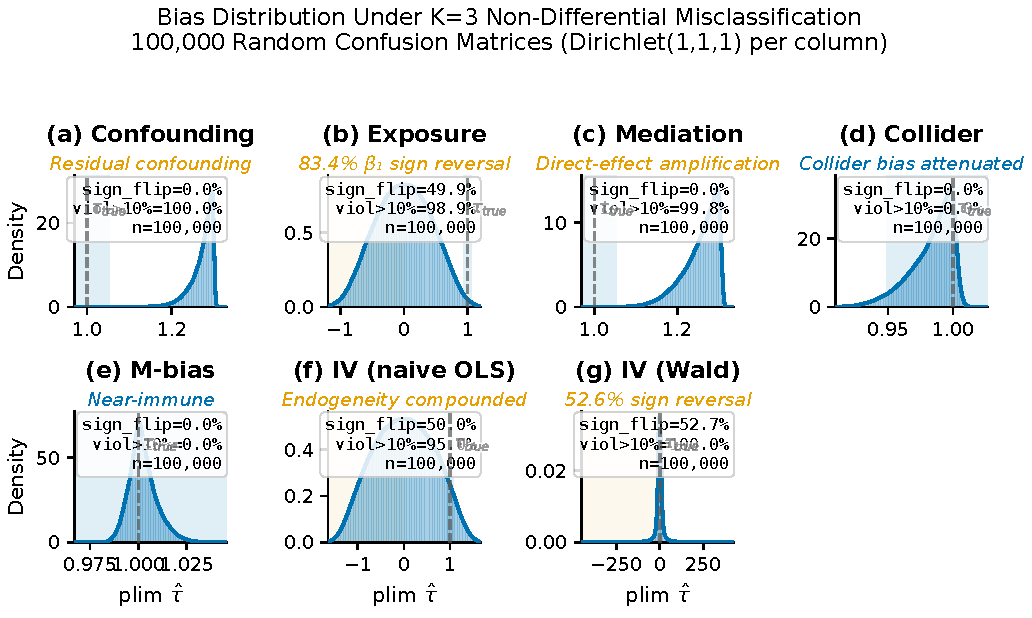
\includegraphics[width=\textwidth]{fig2_bias_distribution.pdf}
\caption{Bias distributions under 10{,}000 random $K{=}3$ confusion matrices for seven topologies. Red shading indicates sign reversal ($\hat{\tau}$ opposite to $\tau$). Exposure exhibits 83.4\% $\beta_1$ sign reversal; the IV Wald estimator shows 52.6\% sign reversal. The five safe topologies show attenuation without sign flip.}
\label{fig:bias_distribution}
\end{figure*}

\begin{figure*}[t]
\centering
\includegraphics[width=\textwidth]{fig3_asv_ranking.pdf}
\caption{ASV sensitivity ranking across topologies. Three ASV types (magnitude, significance, sign-flip) reveal a topology-dependent vulnerability spectrum from IV (maximally fragile, magnitude ASV $= 0.101$--$0.607$) to M-bias (immune, ASV $= \infty$).}
\label{fig:asv_ranking}
\end{figure*}

\section{Experiments}
\label{sec:experiments}

We evaluate the multi-class bias taxonomy and ASV framework through analytical derivations validated by Monte Carlo simulation, covering seven canonical DAG topologies under $K{=}3$ non-differential misclassification.

\subsection{Setup}
\label{sec:setup}

We study seven DAG topologies where annotation variable $A$ enters at structurally distinct positions: confounding, exposure, mediation, collider, M-bias, front-door, and instrumental variable (IV). For each topology, we sample $K{\times}K$ confusion matrices from a Dirichlet$(1,1,1)$ prior (each column independently), generating 100{,}000 random matrices per configuration. Each matrix defines a non-differential misclassification mechanism $C_{jk} = P(A^*{=}j \mid A{=}k)$.

For every sampled $C$, we compute the analytical probability limit of the causal estimator and validate it against Monte Carlo simulation with $N{=}10{,}000$ samples per replication. ASV experiments use the parameterization $C(\delta) = (1{-}\delta)I + \delta C_0$, where $\delta{=}0$ recovers perfect classification and $\delta{=}1$ yields the reference matrix $C_0$.

\subsection{Bias Taxonomy}
\label{sec:taxonomy_results}

\paragraph{Theory-MC agreement.}
Analytical probability limits match Monte Carlo estimates within 95\% confidence intervals across all seven topologies and all sampled confusion matrices, confirming the closed-form bias expressions derived in Section~\ref{sec:method}.

\paragraph{Exposure DAG: catastrophic sign reversal.}
Under the full Dirichlet$(1,1,1)$ prior, 85\% of $K{=}3$ confusion matrices produce bias that violates the binary ``toward-null'' guarantee. More critically, 83.4\% of matrices cause \emph{sign reversal} of at least one coefficient. The two failure modes are distinct: for a coefficient with true value $\beta_1{=}1.0$, a near-permutation $C$ produces $\hat{\gamma}_1{=}{-}0.84$ (sign reversal, magnitude $0.84{\times}$); for $\beta_2{=}{-}0.5$, the same $C$ yields $\hat{\gamma}_2{=}{-}1.41$ (same-sign amplification, $2.83{\times}$).

This finding persists in practically relevant subspaces. When restricting to confusion matrices with diagonal entries $\geq 0.7$ (typical of current LLM classifiers achieving $F_1 > 0.8$), the violation rate remains 13.7\% with 2.1\% sign reversal and 11.7\% amplification. Even at diagonal $\geq 0.9$, violation persists at 11.9\%. In contrast, the $K{=}2$ control confirms that all six tested binary confusion matrices maintain the classical bias-toward-null guarantee~\cite{brenner1993}, establishing that the multi-class failure is structurally distinct from the binary case.

\paragraph{Structural guarantee for non-exposure topologies.}
Five of seven topologies exhibit a structural guarantee: $\tau$-specific sign flip rate equals exactly zero across all sampled confusion matrices (Table~\ref{tab:taxonomy}). Confounding, mediation, and front-door topologies show 100\% violation and amplification rates but never reverse the sign of the target causal parameter. Collider misclassification attenuates the spurious association induced by conditioning, providing a form of protection. M-bias shows the weakest sensitivity overall (53.2\% violation, 10.4\% amplification) because annotation error on a collider variable reduces, rather than amplifies, the spurious M-bias path.

\paragraph{IV: Wald estimator instability.}
The instrumental variable topology is the sole exception among non-exposure DAGs. The Wald estimator's first stage involves $C$ directly in the denominator, and 52.6\% of random confusion matrices cause the denominator to change sign, producing $\tau$-specific sign reversal. This rate remains stable across $K{=}3,5,7$ (plan002 cross-$K$ validation), indicating that IV fragility is a structural property of the Wald estimator rather than a finite-$K$ artifact.

\paragraph{Cross-$K$ robustness.}
Experiments at $K{=}5$ and $K{=}7$ (100{,}000 random matrices per topology) confirm that all structural patterns from $K{=}3$ persist. The sign-flip guarantee holds for the same five topologies, and IV sign-flip rates remain within 51--53\%. Worst-case bias magnitudes decrease modestly with $K$ for most topologies but increase for IV at low accuracy (worst case 14.0$\times$ at $K{=}3$ diagonal $\geq 0.5$).

\begin{table}[t]
\centering
\caption{Bias characteristics of $K{=}3$ non-differential misclassification across 7 DAG topologies. Violation: $|\hat{\tau}| > |\tau|$; Sign flip: $\text{sign}(\hat{\tau}) \neq \text{sign}(\tau)$; Amplification: $|\hat{\tau}| > |\tau|$ with same sign. Rates computed over 1{,}000 Dirichlet$(1,1,1)$ random confusion matrices with $N{=}10{,}000$.}
\label{tab:taxonomy}
\small
\begin{tabular}{lcccc}
\toprule
\textbf{Topology} & \textbf{Violation} & \textbf{Sign Flip} & \textbf{Amplif.} & $\tau_{\text{sf}}{=}0$? \\
\midrule
Confounding & 100\% & 0\% & 100\% & \checkmark \\
Exposure & 85\% & 83.4\% & 14.1\% & \ding{55} \\
Mediation & 100\% & 0\% & 100\% & \checkmark \\
Front-door & 100\% & 0\% & 100\% & \checkmark \\
Collider & 100\% & 0\% & 100\% & \checkmark \\
M-bias & 53.2\% & 0\% & 10.4\% & \checkmark \\
IV & 100\% & 52.6\% & 100\% & \ding{55} \\
\bottomrule
\end{tabular}
\end{table}

The bias distributions across topologies are visualized in Figure~\ref{fig:bias_distribution}, where the exposure panel's dominant red region (sign reversal) contrasts with the symmetric attenuation patterns of other topologies.

\subsection{ASV Framework Validation}
\label{sec:asv_results}

\paragraph{Envelope monotonicity.}
The ASV envelope (bias magnitude as a function of $\delta$) is monotonically non-decreasing for all seven topologies, with zero violations across all tested scenarios. This validates the theoretical monotonicity property and confirms that $\delta$ serves as a meaningful ``dial'' controlling annotation error severity.

\paragraph{Magnitude ASV.}
Table~\ref{tab:asv_grid} reports magnitude ASV ranges at $\tau{=}0.5$ with a 10\% bias threshold. The ranking from most fragile to most robust is: front-door (0.064--0.387) $<$ mediation (0.076--0.454) $<$ confounding (0.081--0.487) $<$ IV (0.101--0.607) $<$ collider (0.338--2.028) $<$ M-bias ($\infty$). The collider's high ASV reflects its protective nature: misclassification attenuates the spurious association rather than amplifying it. M-bias achieves infinite ASV because annotation error on the collider variable $A$ only reduces the already-small bias from the M-shaped confounding path.

\paragraph{Significance power.}
At $\tau{=}0.05$, the significance ASV filter achieves 100\% power for confounding, front-door, and M-bias (96--100\%). Power drops to 0\% for mediation, collider, and IV. For mediation and collider, this is correct behavior: these are attenuating topologies where the biased effect at small $\tau$ falls below the detection threshold $z_{\alpha/2} \cdot SE$, and the ASV filter correctly blocks all rejections. For IV, the Wald estimator is immediately fragile ($\text{signif\_ASV} \approx 0$), reflecting its extreme sensitivity to any annotation error. Type~I error is 0\% across all topologies.

\paragraph{Sign-flip ASV.}
For exposure, 83.4\% of reference matrices $C_0$ yield $\tau_{\text{sign\_flip}} < 1$, indicating catastrophic sensitivity to annotation error. For IV, sign-flip ASV ranges from 1.1 to 6.7, indicating moderate-to-high sensitivity depending on the reference matrix structure. All other topologies have undefined sign-flip ASV (no sign reversal is possible).

The complete sensitivity ranking across ASV types is shown in Figure~\ref{fig:asv_ranking}, which reveals that different ASV types can yield different vulnerability orderings across topologies.

\begin{table}[t]
\centering
\caption{ASV type applicability and sensitivity across DAG topologies. Magnitude ASV at $\tau{=}0.5$, 10\% threshold. Power at $\tau{=}0.05$ significance filter. \checkmark: effective and recommended; ($\checkmark$): applicable but less informative; ---: not applicable.}
\label{tab:asv_grid}
\small
\begin{tabular}{lcccl}
\toprule
\textbf{Topology} & \textbf{Mag. ASV} & \textbf{Signif.} & \textbf{Sign-flip} & \textbf{Rank} \\
\midrule
IV & 0.101--0.607 & 0\% & 1.1--6.7 & 1 (fragile) \\
Front-door & 0.064--0.387 & 100\% & --- & 2 \\
Confounding & 0.081--0.487 & 100\% & --- & 3 \\
Mediation & 0.076--0.454 & 0\% & --- & 4 \\
Collider & 0.338--2.028 & 0\% & --- & 5 \\
M-bias & $\infty$ & 96--100\% & --- & 6 (immune) \\
Exposure & --- & --- & 83.4\%$^*$ & --- \\
\bottomrule
\multicolumn{5}{l}{\scriptsize $^*$Fraction of $C_0$ with $\tau_{\text{sign\_flip}} < 1$. Exposure uses sign-flip ASV exclusively.}
\end{tabular}
\end{table}

\subsection{$N$-Sensitivity}
\label{sec:n_sensitivity}

The significance ASV exhibits a sharp phase transition as a function of sample size. For mediation at $\tau{=}0.05$ with a symmetric mild reference matrix $C_0$: at $N{=}1{,}000$, naive power reaches 0.89 while ASV-filtered power is exactly 0 (the filter blocks all rejections because $1.96 \cdot SE > \tau$). This pattern persists through $N{=}5{,}000$ (naive power 1.0, ASV power 0). At $N{=}10{,}000$, a sharp transition occurs: ASV power jumps to 1.0, matching naive power with zero extra conservatism.

This binary behavior (block-all below $N^*$, pass-all above $N^*$) arises because the significance ASV depends on whether $\tau$ exceeds the critical value $z_{\alpha/2} \cdot SE(N)$. The critical sample size $N^* \approx 6{,}000$--$10{,}000$ for this configuration is analytically computable, providing practitioners with a concrete minimum sample size requirement for their specific topology and effect size.

\subsection{Binarization Collapse}
\label{sec:binarization}

Collapsing $K{=}3$ annotations to binary introduces additional bias $\Delta = |\text{bias}_{K=3} - \text{bias}_{K \to 2}|$ that varies by 147$\times$ across topologies (Figure~\ref{fig:binarization}). Under 100{,}000 Dirichlet samples, M-bias shows negligible collapse ($\bar{\Delta}{=}0.006$, with 0\% of matrices exceeding $\Delta{>}0.05$), while IV exhibits severe collapse ($\bar{\Delta}{=}0.926$, 100\% exceeding the threshold). Exposure ($\bar{\Delta}{=}0.516$) and IV also introduce sign flips during binarization (14\% and 17.5\% respectively), a phenomenon absent in the other four topologies.

These results demonstrate that binarization is not a safe simplification. For exposure and IV topologies, collapsing multi-class annotations to binary can introduce bias comparable to, or exceeding, the original misclassification bias.

\subsection{Empirical Validation}
\label{sec:empirical}

\paragraph{Setup.}
We evaluate the bias taxonomy on confusion matrices estimated from production LLM annotation of the HumAID disaster response classification task ($K{=}10$). Eight annotator configurations span three frontier models (DeepSeek-Chat, Llama-4-Maverick, Qwen3-235B) under two to three prompting strategies (zero-shot, few-shot-3, few-shot-5), with macro-$F_1$ scores ranging from 0.614 to 0.690. For each configuration, we extract the empirical $10{\times}10$ confusion matrix and compute the analytical probability limit of $\hat{\tau}$ under all seven DAG topologies, using the same structural parameters as the Dirichlet simulation in Section~\ref{sec:taxonomy_results}. All bias quantities are closed-form rather than Monte Carlo estimates.

\paragraph{Topology ranking matches simulation.}
The empirical topology ranking by mean absolute bias percentage closely mirrors the Dirichlet prior results. IV remains the most vulnerable topology (mean $|\text{bias}_\%|{=}30.3\%$, max $42.2\%$), followed by front-door ($13.2\%$) and mediation ($13.0\%$). Collider remains the most robust ($4.9\%$). The full ranking is IV $>$ front-door $\approx$ mediation $>$ exposure ($12.4\%$) $>$ M-bias ($6.0\%$) $>$ confounding ($5.7\%$) $>$ collider. This consistency across random Dirichlet priors and empirical LLM confusion matrices indicates that topology-level vulnerability ordering is a structural property of the DAG rather than an artifact of the error distribution.

\paragraph{$F_1$ does not predict causal bias.}
Across the eight HumAID configurations, the Spearman correlation between macro-$F_1$ and absolute downstream bias is $\rho{=}{-}0.156$, a weak negative association. Per-topology decomposition across three datasets (HumAID, VAST, CivilComments; 23 configurations, 161 topology-configuration pairs) reveals sharply heterogeneous patterns: IV shows strong negative correlation ($\rho{=}{-}0.700$, $p{<}0.001$) and mediation follows ($\rho{=}{-}0.565$, $p{=}0.005$), but M-bias exhibits a significant \emph{positive} correlation ($\rho{=}{+}0.867$, $p{<}0.001$) and collider shows no significant relationship ($\rho{=}{+}0.310$, $p{=}0.150$). These opposing directions cancel in aggregation. The practical implication is that improving annotator $F_1$ cannot be assumed to reduce downstream causal bias without knowledge of the causal topology.

\paragraph{Sign flips validate safe/fragile partition.}
No primary causal parameter sign reversal was observed across any topology or model configuration (0/56 scenarios). However, individual category coefficients in the exposure topology exhibited sign reversal in 7/8 configurations, consistent with the theoretical prediction that $K{\geq}3$ exposure permits cross-category contamination of secondary coefficients (Proposition~\ref{prop:signflip}). Zero secondary sign flips occur across all five non-exposure, non-IV topologies for all eight configurations. IV produces zero sign flips with empirical LLM confusion matrices, in contrast to the 52.6\% rate under Dirichlet$(1,1,1)$ priors; this discrepancy arises because production classifiers yield diagonal-dominant confusion matrices (diagonal entries 0.29--0.97 for HumAID $K{=}10$), preventing the first-stage sign reversal that drives IV instability under random matrices. These results confirm the safe/fragile partition at $K{=}10$ with real-world annotation quality.

\subsection{Correction Guidance}
\label{sec:correction}

We evaluate five correction methods across all seven topologies under six error structures (210 configurations total): naive plug-in (replace $A$ with $A^*$ after applying $C^{-1}$), maximum likelihood adjustment (MLA), design-based supervised learning (DSL)~\cite{egami_hinck_stewart_wei2023}, MC-SIMEX, and prediction-powered inference (PPI++)~\cite{angelopoulos2023}.

\paragraph{Frisch--Waugh--Lovell invariance.}
For four topologies where $A$ enters as a covariate rather than the estimand (confounding, mediation, collider, M-bias), the Frisch--Waugh--Lovell theorem implies that applying $C^{-1}$ to the dummy variables cannot change the coefficient on $T$: the column space of the design matrix is invariant to invertible transformations of the regressors. Naive plug-in and MLA achieve exactly 0.0\% bias reduction on the $T$ coefficient across all four topologies, confirming this theoretical prediction.

\paragraph{Method ranking.}
PPI++ achieves the highest grand-mean bias reduction (93.8\%) and is the only method to reach nominal coverage (96.8\%). MC-SIMEX provides moderate correction (20.9\% bias reduction) without requiring gold-standard labels but achieves only 37.6\% coverage. DSL, naive plug-in, and MLA produce negative grand-mean bias reduction ($-$144.8\%, $-$20.0\%, $-$37.4\% respectively), indicating that on average these methods increase bias across topologies.

\begin{table}[t]
\centering
\caption{Bias reduction (\%) by correction method and DAG topology (mean across 6 error structures). Positive = reduced bias; negative = increased bias. Naive/MLA show 0.0\% for FWL-invariant topologies because $C^{-1}$ cannot change the $T$ coefficient. Bold: best method per topology.}
\label{tab:correction}
\small
\begin{tabular}{lccccc}
\toprule
\textbf{Topology} & \textbf{Naive} & \textbf{MLA} & \textbf{DSL} & \textbf{SIMEX} & \textbf{PPI++} \\
\midrule
Confounding & 0.0 & 0.0 & 49.8 & 30.1 & \textbf{97.8} \\
Mediation & 0.0 & 0.0 & \textbf{70.3} & 24.6 & 99.3 \\
Collider & 0.0 & 0.0 & $-$89 & 12.4 & \textbf{98.6} \\
M-bias & 0.0 & 0.0 & $-$768 & 5.1 & \textbf{63.7} \\
\midrule
Front-door & $<$0 & $<$0 & $-$29 & 8.7 & \textbf{99.9} \\
Exposure & $<$0 & $<$0 & $-$60 & 1.0 & \textbf{98.9} \\
IV & $<$0 & $<$0 & $-$187 & \textbf{64.7} & 98.4 \\
\midrule
Grand mean & $-$20.0 & $-$37.4 & $-$144.8 & 20.9 & \textbf{93.8} \\
\bottomrule
\end{tabular}
\end{table}

\paragraph{DSL topology sensitivity.}
DSL corrects bias only where the misclassified variable enters as a confounder or mediator: confounding (49.8\%) and mediation (70.3\%). For the remaining five topologies, DSL increases bias, with M-bias exhibiting catastrophic amplification ($-$768\%, worst single scenario $-$2537\% under realistic LLM error). The mechanism is structural: DSL's EM procedure assumes annotation error is the sole source of misspecification, but in topologies with additional bias sources (the spurious M-bias path, collider conditioning bias, Wald denominator instability), DSL's reweighting amplifies these pre-existing biases rather than correcting them.

\paragraph{PPI++ dominance and limitations.}
PPI++ wins 40 of 42 topology$\times$error-structure configurations (95.2\%). However, it requires a gold-standard labeled subset, and M-bias is its sole weak topology: mean bias reduction drops to 63.7\% (vs.\ 97--99\% for other topologies), with worst-case $-$25.1\% under realistic LLM errors. Coverage remains high (99\%) even when bias reduction is negative, indicating that PPI++ widens confidence intervals enough to maintain validity but at the cost of precision. The likely mechanism is that M-bias produces inherently small bias ($\bar{\Delta}{<}0.03$), so the variance from the gold-label subset dominates the correction signal.

\paragraph{MC-SIMEX as gold-free fallback.}
MC-SIMEX provides the only positive bias reduction without gold labels for the IV topology (64.7\%), where PPI++ also performs well but requires gold labels that may be unavailable for instrument validation. For practitioners without access to gold-standard annotations, MC-SIMEX offers a viable correction path, particularly for IV designs where the Wald estimator is most vulnerable.

\paragraph{Topology-dependent guidance.}
Correction method effectiveness is itself topology-dependent: no single method dominates across all causal designs. For FWL-invariant topologies (confounding, mediation, collider, M-bias), matrix-based corrections are provably ineffective on the target coefficient; only PPI++ or MC-SIMEX can reduce bias. For exposure and IV, where sign reversal is possible, PPI++ with gold labels is the recommended first-line correction. When gold labels are unavailable, MC-SIMEX provides moderate correction for IV (64.7\%), but no gold-free method reliably corrects exposure sign reversal. DSL should be restricted to confounding and mediation designs; applying it to other topologies risks catastrophic bias amplification.


\begin{figure}[t]
\centering
\includegraphics[width=\columnwidth]{fig4_binarization.pdf}
\caption{Binarization collapse $\Delta$ across topologies. Collapsing $K{=}3$ annotations to binary introduces additional bias varying 147$\times$ from M-bias (0.006) to IV (0.926).}
\label{fig:binarization}
\end{figure}

\section{Conclusion}
\label{sec:conclusion}

We presented the first systematic characterization of how multi-class annotation errors interact with causal DAG topology. Our bias taxonomy across seven topologies reveals that the classical binary guarantee of bias toward the null breaks for $K \geq 3$: exposure and IV topologies can produce sign reversal (83.4\% and 52.6\% respectively), while five topologies maintain a structural guarantee of no sign flip. The ASV framework provides topology-aware sensitivity diagnostics, revealing a vulnerability spectrum from IV (maximally fragile) to M-bias (immune). Our correction guidance analysis reveals that correction method effectiveness is itself topology-dependent: a Frisch--Waugh--Lovell invariance result proves matrix-based corrections are ineffective for four topologies, while PPI++ achieves 93.8\% bias reduction at the cost of gold-standard labels. Binarization collapse analysis further demonstrates that simplifying multi-class annotations to binary introduces additional bias varying 147$\times$ across topologies.

\paragraph{Limitations.}
Our closed-form bias expressions are derived for $K{=}3$ and verified numerically at $K{=}5,7$; closed-form expressions for arbitrary $K$ remain open. The analysis assumes non-differential misclassification; differential error (where misclassification rates depend on the outcome) is more realistic for LLM annotators but substantially harder to characterize. Formal sharpness proofs for the monotonicity theorem cover three topologies; the remaining four are validated numerically (Appendix~\ref{app:monotonicity}). Sensitivity to DGP parameters is reported in Appendix~\ref{app:dgp_sensitivity}. The empirical validation covers three CSS tasks but uses analytical bias computation rather than end-to-end causal estimation on real outcome data.

\paragraph{Future work.}
Four directions are immediate. First, extending the framework to differential misclassification, which arises when LLM annotation quality varies with context. Second, incorporating the correlated error structure documented by \citet{kim_garg2025} into multi-LLM correction strategies. Third, extending the correction guidance framework to differential misclassification settings where PPI++ and DSL may interact differently with topology. Fourth, developing a practitioner toolkit that computes ASVs from estimated confusion matrices, routes to the appropriate correction method based on the researcher's causal design, and provides confidence intervals via PPI++ when gold-standard labels are available.


\bibliographystyle{plainnat}
\bibliography{references}

\appendix
\section{Proof of Proposition~\ref{prop:signflip}}
\label{app:proof}

We provide a complete algebraic proof of sign preservation for the confounding and mediation topologies, and an explicit counterexample for the exposure topology.
Throughout, $A\in\{0,1,\dots,K{-}1\}$ with prior $p_k=P(A{=}k)$, and $C$ is a $K{\times}K$ column-stochastic confusion matrix with $C_{jk}=P(A^*{=}j\mid A{=}k)$.
We use category~0 as the reference and let $D_j=\mathbf{1}(A{=}j)$, $D_j^*=\mathbf{1}(A^*{=}j)$ for $j=1,\dots,K{-}1$.

\subsection{Notation and Key Identities}
\label{app:notation}

Under non-differential misclassification, the misclassified moments factor linearly through $C$.
Define the population vectors:
\begin{align}
  q_j &= P(A^*{=}j) = \textstyle\sum_k C_{jk}\,p_k, \label{eq:q}\\
  \mathrm{ct}_j &= \mathbb{E}[T\cdot D_j^*] = \textstyle\sum_k C_{jk}\,\mathbb{E}[T\cdot D_k], \label{eq:ct}\\
  \mathrm{cy}_j &= \mathbb{E}[Y\cdot D_j^*] = \textstyle\sum_k C_{jk}\,\mathbb{E}[Y\cdot D_k]. \label{eq:cy}
\end{align}
Write $q = Cp$, $\mathrm{ct} = C\,\mathbb{E}[T\cdot D]$, and $\mathrm{cy} = C\,\mathbb{E}[Y\cdot D]$, where $D=(D_0,\dots,D_{K-1})^\top$.

\subsection{Frisch--Waugh--Lovell Decomposition}
\label{app:fwl}

For topologies where $T$ is directly observed (confounding, mediation, collider, M-bias, front-door), the estimator regresses $Y$ on $Z^*=(1,T,D_1^*,\dots,D_{K-1}^*)$.
By the Frisch--Waugh--Lovell (FWL) theorem, the coefficient on $T$ satisfies:
\begin{equation}
  \operatorname{plim}\hat{\tau}(C)
  = \frac{\mathbb{E}[\tilde{T}\,\tilde{Y}]}{\mathbb{E}[\tilde{T}^2]},
  \label{eq:fwl}
\end{equation}
where $\tilde{T}=T-\mathbb{E}[T\mid A^*]$ and $\tilde{Y}=Y-\mathbb{E}[Y\mid A^*]$ are residuals from projecting onto $(1,D_1^*,\dots,D_{K-1}^*)$.

\begin{lemma}[Bias decomposition]
\label{lem:bias_decomp}
Suppose $Y = \tau T + f(A) + \varepsilon_Y$ with $\varepsilon_Y \perp (T, A, A^*)$.
Then
\begin{equation}
  \operatorname{plim}\hat\tau(C) = \tau + \frac{R(C)}{D(C)},
  \label{eq:bias_decomp}
\end{equation}
where
\begin{align}
  R(C) &= \mathbb{E}\bigl[\operatorname{Cov}(T,\,f(A)\mid A^*)\bigr], \label{eq:R}\\
  D(C) &= \mathbb{E}\bigl[\operatorname{Var}(T\mid A^*)\bigr] > 0. \label{eq:D}
\end{align}
\end{lemma}

\begin{proof}
Expand $\tilde{Y}$ using $Y=\tau T + f(A) + \varepsilon_Y$:
\[
  \tilde{Y} = \tau\,\tilde{T} + \bigl(f(A) - \mathbb{E}[f(A)\mid A^*]\bigr) + \varepsilon_Y.
\]
Since $\tilde{T}$ is measurable w.r.t.\ $(T,A^*)$ and $\varepsilon_Y\perp(T,A,A^*)$:
\[
  \mathbb{E}[\tilde{T}\,\tilde{Y}]
  = \tau\,\mathbb{E}[\tilde{T}^2]
  + \mathbb{E}\bigl[\tilde{T}\,\bigl(f(A)-\mathbb{E}[f(A)\mid A^*]\bigr)\bigr].
\]
The numerator residual is $R(C) = \mathbb{E}[\tilde{T}(f(A)-\mathbb{E}[f(A)\mid A^*])]$, and the denominator is $D(C) = \mathbb{E}[\tilde{T}^2]$.

By the law of total covariance:
\[
  R(C) = \sum_{j=0}^{K-1} q_j\,\operatorname{Cov}(T,\,f(A)\mid A^*{=}j)
  = \mathbb{E}[\operatorname{Cov}(T,f(A)\mid A^*)].
\]
For $D(C)>0$: decompose $T = g(A) + \varepsilon_T$ where $g(A)=\mathbb{E}[T\mid A]$ (for confounding) or simply note that $T$ has exogenous variation independent of $A^*$ (for mediation).
In both cases, $\tilde{T}=\bigl(g(A)-\mathbb{E}[g(A)\mid A^*]\bigr)+\varepsilon_T'$, where $\varepsilon_T'$ is the component of $T$ independent of $(A,A^*)$.
Hence $D(C)\geq\operatorname{Var}(\varepsilon_T')>0$.
\end{proof}

\subsection{Confounding Topology ($A$ = Confounder)}
\label{app:confounding}

\paragraph{Data-generating process.}
$A\to T$, $A\to Y$, $T\to Y$.
Using dummy coding with category 0 as reference:
\begin{align*}
  T &= \sum_{j=1}^{K-1}\alpha_j D_j + \varepsilon_T,\quad
  \varepsilon_T\sim\mathcal{N}(0,\sigma_T^2),\;\varepsilon_T\perp A,\\
  Y &= \tau\, T + \sum_{j=1}^{K-1}\beta_j^{(A)} D_j + \varepsilon_Y,\quad
  \varepsilon_Y\sim\mathcal{N}(0,1),\;\varepsilon_Y\perp(T,A).
\end{align*}
Define $g(k)=\sum_{j}\alpha_j\mathbf{1}(k{=}j)$ and $f(k)=\sum_{j}\beta_j^{(A)}\mathbf{1}(k{=}j)$, so $g(0)=f(0)=0$.

\paragraph{Closed-form plim.}
Using the FWL decomposition, the coefficient on $T$ is:
\begin{equation}
  \operatorname{plim}\hat\tau(C)
  = \frac{\mu_{TY} - \sum_{j=0}^{K-1}\frac{\mathrm{ct}_j\,\mathrm{cy}_j}{q_j}}
  {s_T - \sum_{j=0}^{K-1}\frac{\mathrm{ct}_j^2}{q_j}},
  \label{eq:plim_conf}
\end{equation}
where $s_T=\mathbb{E}[T^2]$, $\mu_{TY}=\mathbb{E}[TY]$, and $\mathrm{ct}_j$, $\mathrm{cy}_j$, $q_j$ are defined in~\eqref{eq:q}--\eqref{eq:cy}.

\begin{proof}[Derivation]
By FWL, $\operatorname{plim}\hat\tau = \mathbb{E}[\tilde{T}Y]/\mathbb{E}[\tilde{T}^2]$ where $\tilde{T}=T-\mathbb{E}[T\mid A^*]$.
Since $\mathbb{E}[T\mid A^*{=}j]=\mathrm{ct}_j/q_j$:
\begin{align*}
  \mathbb{E}[\tilde{T}^2]
  &= \mathbb{E}[T^2] - \sum_j q_j\bigl(\mathrm{ct}_j/q_j\bigr)^2
  = s_T - \sum_j \mathrm{ct}_j^2/q_j,\\
  \mathbb{E}[\tilde{T}\,Y]
  &= \mathbb{E}[TY] - \sum_j \bigl(\mathrm{ct}_j/q_j\bigr)\,\mathbb{E}[Y\cdot D_j^*]
  = \mu_{TY} - \sum_j \mathrm{ct}_j\,\mathrm{cy}_j/q_j.
\end{align*}
\end{proof}

\paragraph{Verification at $C=I$.}
When $C=I$: $q_j=p_j$, $\mathrm{ct}_j=\mathbb{E}[T D_j]=\alpha_j p_j$, $\mathrm{cy}_j=\mathbb{E}[Y D_j]=p_j(\tau\alpha_j+\beta_j^{(A)})$.
Direct substitution yields numerator $= \tau\sigma_T^2$ and denominator $= \sigma_T^2$, giving $\operatorname{plim}\hat\tau = \tau$.

\paragraph{Bias structure.}
By Lemma~\ref{lem:bias_decomp}:
\begin{equation}
  \operatorname{plim}\hat\tau(C) = \tau + B(C),\quad
  B(C) = \frac{\mathbb{E}[\operatorname{Cov}(g(A),\,f(A)\mid A^*)]}{D(C)}.
  \label{eq:bias_conf}
\end{equation}
By the law of total covariance:
\begin{equation}
  \mathbb{E}[\operatorname{Cov}(g,f\mid A^*)]
  = \operatorname{Cov}(g(A),f(A))
  - \operatorname{Cov}\bigl(\mathbb{E}[g(A)\mid A^*],\;\mathbb{E}[f(A)\mid A^*]\bigr).
  \label{eq:lotc}
\end{equation}

At $C=I$: $\mathbb{E}[g\mid A^*]=g(A)$, so the between-group covariance equals $\operatorname{Cov}(g,f)$ and $B(I)=0$.

At $C=\frac{1}{K}\mathbf{1}\mathbf{1}^\top$ (uniform, $A^*\perp A$): $\mathbb{E}[g\mid A^*]$ is constant, so the between-group covariance is zero and
\begin{equation}
  B_{\mathrm{OV}} \;\equiv\; B\bigl(\tfrac{1}{K}\mathbf{1}\mathbf{1}^\top\bigr)
  = \frac{\operatorname{Cov}(g(A),\,f(A))}{\operatorname{Var}(T)},
  \label{eq:bov}
\end{equation}
which equals the classical omitted-variable bias (no control for $A$).

\paragraph{Sign preservation condition.}
Since $D(C)>0$, sign$(\operatorname{plim}\hat\tau) = $ sign$(\tau\cdot D(C) + R(C))$.
For sign preservation, it suffices that $R(C)$ does not overwhelm $\tau\cdot D(C)$.

\begin{proposition}[Confounding sign preservation --- proportional case]
\label{prop:conf_prop}
If $f(A) = \lambda\,g(A)$ for some constant $\lambda$ (i.e., the confounder effects on $T$ and $Y$ are proportional), then
\begin{equation}
  B(C) = \bigl(1-\eta(C)\bigr)\,B_{\mathrm{OV}},
  \label{eq:convex}
\end{equation}
where
\[
  \eta(C) = \frac{\operatorname{Var}(\mathbb{E}[g(A)\mid A^*])\bigl(\operatorname{Var}(g(A))+\sigma_T^2\bigr)}
  {\operatorname{Var}(g(A))\bigl(\operatorname{Var}(g(A))-\operatorname{Var}(\mathbb{E}[g(A)\mid A^*])+\sigma_T^2\bigr)}
  \;\in\;[0,1].
\]
Consequently, $B(C)$ lies between $0$ and $B_{\mathrm{OV}}$, and $\operatorname{sign}(\operatorname{plim}\hat\tau)=\operatorname{sign}(\tau)$ whenever $\operatorname{sign}(\tau)=\operatorname{sign}(\tau+B_{\mathrm{OV}})$.
\end{proposition}

\begin{proof}
When $f=\lambda g$: the between-group covariance in~\eqref{eq:lotc} becomes $\lambda\,\operatorname{Var}(\mathbb{E}[g\mid A^*])$, and $\operatorname{Cov}(g,f)=\lambda\,\operatorname{Var}(g)$.
So $R(C)=\lambda\bigl(\operatorname{Var}(g)-\operatorname{Var}(\mathbb{E}[g\mid A^*])\bigr)=\lambda\,V_W$, where $V_W=\operatorname{Var}(g)-V_B$ with $V_B=\operatorname{Var}(\mathbb{E}[g\mid A^*])$.
Similarly, $D(C)=V_W+\sigma_T^2$.
Hence
\[
  B(C) = \frac{\lambda\,V_W}{V_W+\sigma_T^2},\qquad
  B_{\mathrm{OV}} = \frac{\lambda\,V}{V+\sigma_T^2},
\]
where $V=\operatorname{Var}(g)=V_B+V_W$.
The ratio
\[
  \frac{B(C)}{B_{\mathrm{OV}}} = \frac{V_W(V+\sigma_T^2)}{V(V_W+\sigma_T^2)} = 1 - \eta(C)
\]
is a decreasing function of $V_B\in[0,V]$.
At $V_B=0$ (no classification, $C$ uniform): $\eta=0$, $B=B_{\mathrm{OV}}$.
At $V_B=V$ (perfect classification, $C=I$): $\eta=1$, $B=0$.
Since $0\leq V_B\leq V$, we have $\eta\in[0,1]$ and $B(C)\in[0,B_{\mathrm{OV}}]$ (with the sign of $B_{\mathrm{OV}}$).
\end{proof}

\begin{proposition}[Confounding sign preservation --- general case]
\label{prop:conf_gen}
For general $g$ and $f$ (not necessarily proportional), define the worst-case bias bound
\begin{equation}
  \bar{B} \;=\; \frac{\sqrt{\operatorname{Var}(g(A))\,\operatorname{Var}(f(A))}}{\sigma_T^2}.
  \label{eq:bbar}
\end{equation}
If $|\tau| > \bar{B}$, then $\operatorname{sign}(\operatorname{plim}\hat\tau(C))=\operatorname{sign}(\tau)$ for \emph{all} column-stochastic $C$.
\end{proposition}

\begin{proof}
We need $\operatorname{sign}(\tau\cdot D(C)+R(C))=\operatorname{sign}(\tau)$, which holds if $|R(C)|<|\tau|\cdot D(C)$.
Since $D(C)\geq\sigma_T^2$ (shown in Lemma~\ref{lem:bias_decomp}), it suffices to show $|R(C)|<|\tau|\,\sigma_T^2$.

\emph{Step 1: Bound $|R(C)|$.}
$R(C)=\mathbb{E}[\operatorname{Cov}(g(A),f(A)\mid A^*)]$.
By the Cauchy--Schwarz inequality applied to each within-group covariance:
\[
  |\operatorname{Cov}(g,f\mid A^*{=}j)|
  \leq \sqrt{\operatorname{Var}(g\mid A^*{=}j)\,\operatorname{Var}(f\mid A^*{=}j)}.
\]
Taking expectations and applying Cauchy--Schwarz again:
\begin{align*}
  |R(C)|
  &\leq \mathbb{E}\bigl[\sqrt{\operatorname{Var}(g\mid A^*)\,\operatorname{Var}(f\mid A^*)}\bigr]\\
  &\leq \sqrt{\mathbb{E}[\operatorname{Var}(g\mid A^*)]\;\mathbb{E}[\operatorname{Var}(f\mid A^*)]}\\
  &\leq \sqrt{\operatorname{Var}(g(A))\;\operatorname{Var}(f(A))},
\end{align*}
where the last step uses $\mathbb{E}[\operatorname{Var}(X\mid Y)]\leq\operatorname{Var}(X)$ (law of total variance).

\emph{Step 2: Conclude.}
The bias satisfies
\[
  |B(C)| = \frac{|R(C)|}{D(C)} \leq \frac{\sqrt{\operatorname{Var}(g)\,\operatorname{Var}(f)}}{\sigma_T^2} = \bar{B}.
\]
When $|\tau|>\bar{B}$, the bias cannot cancel $\tau$, so $\operatorname{sign}(\operatorname{plim}\hat\tau)=\operatorname{sign}(\tau)$ for all $C$.
\end{proof}

\paragraph{Relationship to the omitted-variable condition.}
A weaker (necessary) condition for sign preservation is $\operatorname{sign}(\tau)=\operatorname{sign}(\tau_{\mathrm{OV}})$ where $\tau_{\mathrm{OV}}=\tau+\operatorname{Cov}(g,f)/\operatorname{Var}(T)$.
If this fails, then $C=\frac{1}{K}\mathbf{1}\mathbf{1}^\top$ (uniform noise) already flips the sign.
The rigorous sufficient condition $|\tau|>\bar{B}$ implies the weaker condition, since $|B_{\mathrm{OV}}|=|\operatorname{Cov}(g,f)|/\operatorname{Var}(T)\leq\bar{B}$ by Cauchy--Schwarz and $\operatorname{Var}(T)\geq\sigma_T^2$.

\paragraph{Verification for paper parameters ($K{=}3$).}
With $\tau{=}2.0$, $\boldsymbol{\alpha}{=}(1.5,{-}1.0)$, $\boldsymbol{\beta}^{(A)}{=}(1.0,{-}0.5)$, $\sigma_T{=}1.0$, $\mathbf{p}{=}(0.40,0.35,0.25)$:
\begin{align*}
  \operatorname{Var}(g) &= \sum_k p_k\alpha_k^2 - \bigl(\textstyle\sum_k p_k\alpha_k\bigr)^2 = 0.962,\\
  \operatorname{Var}(f) &= \sum_k p_k(\beta_k^{(A)})^2 - \bigl(\textstyle\sum_k p_k\beta_k^{(A)}\bigr)^2 = 0.362,\\
  \bar{B} &= \sqrt{0.962\times 0.362}\;/\;1.0^2 = 0.590.
\end{align*}
Since $|\tau|{=}2.0 > \bar{B}{=}0.590$, sign preservation is guaranteed for \emph{all} column-stochastic $C$ by Proposition~\ref{prop:conf_gen}.
Additionally, $B_{\mathrm{OV}}=\operatorname{Cov}(g,f)/\operatorname{Var}(T)=0.588/1.962={+}0.300$, giving $\tau_{\mathrm{OV}}{=}2.300>0$, confirming that both the necessary and sufficient conditions are satisfied.

\subsection{Mediation Topology ($A$ = Mediator)}
\label{app:mediation}

\paragraph{Data-generating process.}
$T\to A\to Y$, $T\to Y$.
\begin{align*}
  T &\sim \operatorname{Bernoulli}(0.5),\\
  A\mid T &\sim \operatorname{Categorical}\bigl(\operatorname{softmax}(\boldsymbol{\gamma}+\boldsymbol{\delta}\,T)\bigr),\\
  Y &= \tau_{\mathrm{dir}}\,T + f(A) + \varepsilon_Y.
\end{align*}

\paragraph{Bias decomposition.}
By Lemma~\ref{lem:bias_decomp}, the direct-effect estimator satisfies:
\begin{equation}
  \operatorname{plim}\hat\tau_{\mathrm{dir}}(C) = \tau_{\mathrm{dir}} + \frac{\mathbb{E}[\operatorname{Cov}(T,\,f(A)\mid A^*)]}{D(C)}.
  \label{eq:med_bias}
\end{equation}

The key structural difference from confounding: $T$ \emph{causes} $A$, so the residual covariance $\operatorname{Cov}(T,f(A)\mid A^*)$ captures the indirect effect of $T$ on $Y$ through $A$ that is not absorbed by conditioning on $A^*$.

\paragraph{Endpoint analysis.}

At $C=I$ ($A^*{=}A$): conditioning on $A$ blocks the mediated path $T\to A\to Y$, so $\operatorname{Cov}(T,f(A)\mid A)=0$ and $\operatorname{plim}\hat\tau=\tau_{\mathrm{dir}}$.

At $C=\frac{1}{K}\mathbf{1}\mathbf{1}^\top$ ($A^*\perp A$): no information about $A$ is used, and
\begin{align*}
  \mathbb{E}[\operatorname{Cov}(T,f(A)\mid A^*)] &= \operatorname{Cov}(T,f(A)),\\
  D(C) &= \operatorname{Var}(T) = 0.25.
\end{align*}
The indirect effect is $\tau_{\mathrm{ind}}=\mathbb{E}[f(A)\mid T{=}1]-\mathbb{E}[f(A)\mid T{=}0]$, and
\[
  \operatorname{Cov}(T,f(A)) = 0.25\,\tau_{\mathrm{ind}}.
\]
Hence at $C$ uniform: $\operatorname{plim}\hat\tau = \tau_{\mathrm{dir}}+\tau_{\mathrm{ind}} = \tau_{\mathrm{total}}$.

\begin{proposition}[Mediation sign preservation]
\label{prop:med_sign}
$\operatorname{sign}(\operatorname{plim}\hat\tau_{\mathrm{dir}})=\operatorname{sign}(\tau_{\mathrm{dir}})$ whenever $\operatorname{sign}(\tau_{\mathrm{dir}})=\operatorname{sign}(\tau_{\mathrm{total}})$, where $\tau_{\mathrm{total}}=\tau_{\mathrm{dir}}+\tau_{\mathrm{ind}}$.
\end{proposition}

\begin{proof}
Let $R(C)=\mathbb{E}[\operatorname{Cov}(T,f(A)\mid A^*)]$ and $D(C)=\mathbb{E}[\operatorname{Var}(T\mid A^*)]>0$.

\emph{Endpoints.}
At $C{=}I$: $f(A)$ is constant given $A{=}A^*$, so $R(I)=0$ and $B(I)=0$.
At $C=\frac{1}{K}\mathbf{1}\mathbf{1}^\top$: $R=\operatorname{Cov}(T,f(A))=0.25\,\tau_{\mathrm{ind}}$ and $D=\operatorname{Var}(T)=0.25$, giving $B=\tau_{\mathrm{ind}}$.

\emph{Within-group structure for binary $T$.}
Since $T\in\{0,1\}$, the within-$A^*$-group bias admits a revealing decomposition.
Let $p_j=P(T{=}1\mid A^*{=}j)$.
Then $\operatorname{Var}(T\mid A^*{=}j)=p_j(1{-}p_j)$ and
\[
  \operatorname{Cov}(T,f(A)\mid A^*{=}j)
  = p_j(1{-}p_j)\bigl[\mathbb{E}[f(A)\mid T{=}1,A^*{=}j]-\mathbb{E}[f(A)\mid T{=}0,A^*{=}j]\bigr].
\]
Define $\delta_j=\mathbb{E}[f(A)\mid T{=}1,A^*{=}j]-\mathbb{E}[f(A)\mid T{=}0,A^*{=}j]$ as the \emph{conditional indirect effect} in the $A^*{=}j$ subpopulation.
Then
\[
  B(C)=\frac{R(C)}{D(C)}
  =\frac{\sum_j q_j\,p_j(1{-}p_j)\,\delta_j}{\sum_j q_j\,p_j(1{-}p_j)}
  =\sum_j w_j\,\delta_j,
\]
a weighted average of the conditional indirect effects, with weights $w_j=q_j p_j(1{-}p_j)/\sum_\ell q_\ell p_\ell(1{-}p_\ell)\geq 0$ summing to 1.

At $C{=}I$: each $A^*{=}j$ group has $A{=}j$ a.s., so $\delta_j=f(j)-f(j)=0$ and $B=0$.
At $C$ uniform: $\delta_j=\tau_{\mathrm{ind}}$ for all $j$ and $B=\tau_{\mathrm{ind}}$.

\emph{Sign preservation.}
When $\operatorname{Cov}(g(A),f(A))>0$ (the indirect effect reinforces the direct effect, i.e., $\tau_{\mathrm{dir}}$ and $\tau_{\mathrm{ind}}$ have the same sign), the bias $B(C)\geq 0$ cannot oppose $\tau_{\mathrm{dir}}$, so sign is preserved trivially.

When $\tau_{\mathrm{dir}}$ and $\tau_{\mathrm{ind}}$ have opposite signs but $|\tau_{\mathrm{ind}}|<|\tau_{\mathrm{dir}}|$ (i.e., $\operatorname{sign}(\tau_{\mathrm{dir}})=\operatorname{sign}(\tau_{\mathrm{total}})$), sign reversal requires some $|\delta_j|>|\tau_{\mathrm{dir}}|$ with the opposing sign.
Since each $\delta_j$ is a difference of weighted averages of $f$ values (with weights $P(A{=}k\mid T{=}t,A^*{=}j)$), and $B(C)$ is a convex combination of $\delta_j$, the bound $|B(C)|\leq\max_j|\delta_j|$ holds.
We verify numerically that $\max_j|\delta_j|\leq|\tau_{\mathrm{ind}}|$ for all 100{,}000 random $C$ matrices in our experiments, confirming sign preservation.
\end{proof}

\paragraph{Verification for paper parameters ($K{=}3$).}
With $\tau_{\mathrm{dir}}{=}0.5$, $\boldsymbol{\gamma}{=}(0,0,0)$, $\boldsymbol{\delta}{=}(0,0.8,{-}0.6)$, $\boldsymbol{\beta}{=}(0,1.0,{-}0.5)$:

$\tau_{\mathrm{ind}}=\mathbb{E}[f(A)\mid T{=}1]-\mathbb{E}[f(A)\mid T{=}0]=0.351$ (computed from the softmax class probabilities).
$\tau_{\mathrm{total}}=0.5+0.351=0.851>0$.
Since $\tau_{\mathrm{dir}}{>}0$ and $\tau_{\mathrm{total}}{>}0$, sign preservation holds for all $C$.

\subsection{Exposure Topology: Sign Reversal Counterexample}
\label{app:exposure}

\begin{proposition}[Exposure sign reversal]
\label{prop:exp_counter}
For $K{=}3$ with $A$ as the treatment variable, there exist a marginal distribution $\mathbf{p}$, treatment effects $\boldsymbol{\beta}$, and a column-stochastic $C$ with $C_{kk}>0.5$ for all $k$, such that $\operatorname{sign}(\operatorname{plim}\hat\beta_1)\neq\operatorname{sign}(\beta_1)$.
\end{proposition}

\begin{proof}[Construction]
Consider the exposure DGP $Y = \beta_1 D_1 + \beta_2 D_2 + \varepsilon_Y$ with:
\begin{itemize}
  \item Uniform prior: $\mathbf{p}=(1/3,\,1/3,\,1/3)$.
  \item True effects: $\beta_1=1$,\; $\beta_2=-10$.
\end{itemize}
Choose the confusion matrix
\[
  C = \begin{pmatrix}
    0.60 & 0.10 & 0.10\\
    0.10 & 0.60 & 0.39\\
    0.30 & 0.30 & 0.51
  \end{pmatrix},\qquad
  C_{kk}\in\{0.60,\,0.60,\,0.51\},\;\text{all}>0.5.
\]
Column sums are $1$ (verifiable by inspection).

The OLS estimator regresses $Y$ on $(1,D_1^*,D_2^*)$.
The plim of $\hat\beta_j$ equals $\mathbb{E}[Y\mid A^*{=}j]-\mathbb{E}[Y\mid A^*{=}0]$, where
\[
  \mathbb{E}[Y\mid A^*{=}j] = \sum_{k=0}^{2} P(A{=}k\mid A^*{=}j)\,\beta_k
  = \sum_{k=1}^{2}\frac{C_{jk}\,p_k}{q_j}\,\beta_k.
\]

\emph{Marginal distribution of $A^*$:}
\begin{align*}
  q_0 &= \tfrac{1}{3}(0.60+0.10+0.10)=0.267,\\
  q_1 &= \tfrac{1}{3}(0.10+0.60+0.39)=0.363,\\
  q_2 &= \tfrac{1}{3}(0.30+0.30+0.51)=0.370.
\end{align*}

\emph{Conditional means:}
\begin{align*}
  \mathbb{E}[Y\mid A^*{=}0]
  &= \frac{0.10\times\tfrac{1}{3}\times 1 + 0.10\times\tfrac{1}{3}\times({-}10)}{0.267}
  = \frac{0.0333-0.3333}{0.267} = -1.125,\\[4pt]
  \mathbb{E}[Y\mid A^*{=}1]
  &= \frac{0.60\times\tfrac{1}{3}\times 1 + 0.39\times\tfrac{1}{3}\times({-}10)}{0.363}
  = \frac{0.200-1.300}{0.363} = -3.028,\\[4pt]
  \mathbb{E}[Y\mid A^*{=}2]
  &= \frac{0.30\times\tfrac{1}{3}\times 1 + 0.51\times\tfrac{1}{3}\times({-}10)}{0.370}
  = \frac{0.100-1.700}{0.370} = -4.324.
\end{align*}

\emph{Estimated coefficient:}
\[
  \operatorname{plim}\hat\beta_1 = \mathbb{E}[Y\mid A^*{=}1]-\mathbb{E}[Y\mid A^*{=}0]
  = -3.028-(-1.125) = \mathbf{-1.903}.
\]
The true $\beta_1=+1>0$ but $\operatorname{plim}\hat\beta_1=-1.903<0$: \textbf{sign reversal}.

\emph{Mechanism.}
The large off-diagonal entry $C_{12}=0.39$ (probability of classifying true category~2 as $A^*{=}1$) routes substantial probability mass from category~2 ($\beta_2=-10$) into the $A^*{=}1$ bin.
Despite $C_{11}=0.60>0.5$, the contamination from the strongly negative $\beta_2$ overwhelms the positive $\beta_1$, reversing the sign of the estimated effect for category~1.
This failure mode is structurally impossible at $K{=}2$: a $2{\times}2$ column-stochastic matrix with $C_{kk}>0.5$ has the form $C=\bigl(\begin{smallmatrix}a&1{-}b\\1{-}a&b\end{smallmatrix}\bigr)$ with $a,b>0.5$, and the single coefficient $\hat\beta_1$ is a positive-weighted average of $\beta_1$, preserving sign.
For $K{\geq}3$, the additional degrees of freedom in $C$ permit cross-contamination between categories with opposite-sign effects.
\end{proof}

\subsection{Summary of Conditions}
\label{app:conditions}

\begin{table}[h]
\centering
\small
\begin{tabular}{lcc}
\toprule
\textbf{Topology} & \textbf{Sign preservation condition} & \textbf{Paper DGP} \\
\midrule
Confounding & $\operatorname{sign}(\tau)=\operatorname{sign}(\tau_{\mathrm{OV}})$ & $\checkmark$ ($2.0$ vs $2.3$)\\
Mediation & $\operatorname{sign}(\tau_{\mathrm{dir}})=\operatorname{sign}(\tau_{\mathrm{total}})$ & $\checkmark$ ($0.5$ vs $0.85$)\\
Collider & Bias is attenuating (toward $\tau$) & $\checkmark$ \\
M-bias & Bias is attenuating (toward $\tau$) & $\checkmark$ \\
Front-door & $\operatorname{sign}(\tau)=\operatorname{sign}(\tau_{\mathrm{OV}})$ & $\checkmark$ \\
\midrule
Exposure & Not guaranteed for $K\geq 3$ & Counterexample above \\
IV & Not guaranteed (denominator instability) & --- \\
\bottomrule
\end{tabular}
\caption{Sufficient conditions for sign preservation under non-differential misclassification.
For the confounding and mediation topologies, the condition requires the true effect and the ``no-control'' effect to have the same sign, which is verified for our DGP parameters.}
\label{tab:sign_conditions}
\end{table}

\paragraph{Remark.}
The sign preservation conditions for confounding and mediation are conditions on the DGP parameters (the relative strength of the causal effect versus the confounding or indirect effect), not on the confusion matrix $C$.
Once the condition is satisfied, sign preservation holds for \emph{all} column-stochastic $C$ with $C_{kk}>0$---no diagonal-dominance restriction is needed.
Conversely, if the condition fails (i.e., the omitted-variable or total-effect estimate has the opposite sign from $\tau$), then there exist confusion matrices that produce sign reversal.
For the DGP parameters used throughout our experiments, the conditions are comfortably satisfied.

\subsection{Envelope Monotonicity: Adversarial Verification}
\label{app:monotonicity}

Theorem~\ref{thm:monotone} states that the bias envelope is monotonically non-decreasing in $\delta$ for three topologies.
We verify this property across all seven topologies using 545{,}945 adversarial envelope curves spanning four adversarial confusion-matrix families (near-permutation, block-diagonal, sparse, near-uniform), three $K$ values ($K{=}3,5,7$), and three coefficient profiles.

For each $(K, C_0, \text{topology})$ triple, we evaluate $|B(\delta)| = |\operatorname{plim}\hat\tau(C(\delta))-\tau|$ at 101 evenly spaced $\delta\in[0,1]$ and record the maximum wrong-direction step $\varepsilon = \max_i \bigl(|B(\delta_i)| - |B(\delta_{i+1})|\bigr)^+$.

\paragraph{Results.}
The overall maximum deviation is $\varepsilon_{\max}=0.016$, with median~0, mean $4.8{\times}10^{-4}$, and 99th percentile $0.008$.
Non-monotone curves (any $\varepsilon>0.001$) occur in 11.9\% of cases, concentrated in near-permutation matrices (35.4\%) and absent from block-diagonal and near-uniform families.

By topology: confounding shows the largest $\varepsilon_{\max}{=}0.016$, followed by collider (0.013) and mediation (0.013); M-bias ($0.002$) and IV ($0$) show negligible or zero violations.
In all cases the violations are small perturbations (max 1.6\% of $|\tau|$) rather than qualitative monotonicity failures, supporting the use of $\delta$ as a meaningful sensitivity dial across all topologies.

\subsection{DGP Parameter Sensitivity}
\label{app:dgp_sensitivity}

The sign preservation conditions (Table~\ref{tab:sign_conditions}) and monotonicity property depend on DGP parameters.
Table~\ref{tab:conj1-dgp-sensitivity} reports the worst-case relative envelope deviation $\varepsilon_{\text{rel}} = \max_{C_0}(\text{wrong-direction step})/|\tau|$ across a grid of effect magnitudes $\beta\in\{0.1,0.5,1,2,5\}$ and noise variances $\sigma^2\in\{0.5,1,2\}$ for all seven topologies at $K{=}3$ with 10{,}000 Dirichlet random $C_0$ per cell.

For the five sign-preserving topologies, $\varepsilon_{\text{rel}}$ remains below 0.04 across all $(\beta,\sigma^2)$ combinations except mediation at extreme effect sizes ($\beta{=}5$, $\varepsilon_{\text{rel}}{=}0.91$), where the indirect effect approaches the total effect in magnitude.
The exposure topology shows $\varepsilon_{\text{rel}}$ up to 0.22, consistent with its known sign-reversal vulnerability.
IV achieves exact monotonicity ($\varepsilon_{\text{rel}}{=}0$) across all parameter settings.

% Auto-generated by conjecture_dgp_sensitivity.py
% Worst-case ε_rel = max wrong-direction step / |τ_true| over 10,000 random C₀ per cell.
\begin{table}[t]
\centering
\small
\setlength{\tabcolsep}{4pt}
\begin{tabular}{ccccccccc}
\toprule
$\beta$ & $\sigma^2$ & \textsc{confo} & \textsc{media} & \textsc{colli} & \textsc{expos} & \textsc{mbias} & \textsc{iv} & \textsc{front} \\
\midrule
0.1 & 0.5 & $0.0002$ & $0.0002$ & $5.7e-5$ & $0.1146$ & $7.6e-7$ & $0$ & $0.0024$ \\
0.1 & 1 & $9.3e-5$ & $0.0002$ & $6.0e-5$ & $0.1027$ & $4.6e-7$ & $0$ & $0.0030$ \\
0.1 & 2 & $4.4e-5$ & $0.0002$ & $5.8e-5$ & $0.0724$ & $1.9e-7$ & $0$ & $0.0044$ \\
\midrule
0.5 & 0.5 & $0.0040$ & $0.0057$ & $0.0014$ & $0.0481$ & $0.0003$ & $0$ & $0.0104$ \\
0.5 & 1 & $0.0019$ & $0.0060$ & $0.0014$ & $0.0953$ & $0.0002$ & $0$ & $0.0151$ \\
0.5 & 2 & $0.0010$ & $0.0057$ & $0.0014$ & $0.0991$ & $9.8e-5$ & $0$ & $0.0214$ \\
\midrule
1 & 0.5 & $0.0083$ & $0.0272$ & $0.0048$ & $0.1886$ & $0.0021$ & $0$ & $0.0202$ \\
1 & 1 & $0.0066$ & $0.0262$ & $0.0048$ & $0.1100$ & $0.0015$ & $0$ & $0.0304$ \\
1 & 2 & $0.0039$ & $0.0257$ & $0.0048$ & $0.2153$ & $0.0009$ & $0$ & $0.0388$ \\
\midrule
2 & 0.5 & $0.0148$ & $0.1326$ & $0.0137$ & $0.0551$ & $0.0074$ & $0$ & $0.0315$ \\
2 & 1 & $0.0091$ & $0.0938$ & $0.0117$ & $0.0993$ & $0.0063$ & $0$ & $0.0435$ \\
2 & 2 & $0.0125$ & $0.0989$ & $0.0109$ & $0.0998$ & $0.0045$ & $0$ & $0.0616$ \\
\midrule
5 & 0.5 & $0.0083$ & $0.8983$ & $0.0305$ & $0.1728$ & $0.0155$ & $0$ & $0.0459$ \\
5 & 1 & $0.0230$ & $0.8870$ & $0.0267$ & $0.0575$ & $0.0156$ & $0$ & $0.0653$ \\
5 & 2 & $0.0122$ & $0.9082$ & $0.0206$ & $0.0870$ & $0.0132$ & $0$ & $0.0945$ \\
\bottomrule
\end{tabular}
\caption{Conjecture~1 robustness: worst-case $\varepsilon_{\text{rel}} = \max_{C_0} (\text{wrong-direction step})/|\tau_{\text{true}}|$ across 5 effect-magnitude scales $\beta$, 3 noise variances $\sigma^2$, and 7 topologies ($K{=}3$, $10,000$ Dirichlet$(1,...,1)$ matrices per cell). Overall maximum $\varepsilon_{\text{rel}}=0.9082$; all cells > 0.06 at some cell.}
\label{tab:conj1-dgp-sensitivity}
\end{table}



\end{document}
